\documentclass[12pt]{article}
\usepackage[paper=a4paper, margin=1in]{geometry} 

%Required packages
\usepackage{natbib} 
\usepackage{graphicx}
\usepackage{amsmath}
\usepackage{mathtools}
\usepackage{setspace}
\usepackage[document]{ragged2e}
\usepackage{lineno}
\usepackage{gensymb}
\setcounter{secnumdepth}{-1} 
\raggedright


\begin{document}
\setcounter{page}{1}

\textbf{Title}: What controls the range of hosts a fish parasite infects? \\
\vspace{0.5cm}
\textbf{Authors:} Tad Dallas$^{1,2}$, Andrew Park $^{1}$, and John M. Drake$^{1}$ \\
\vspace{0.5cm}
\textbf{Affiliations}: 
\begin{enumerate}
  \item University of Georgia, Odum School of Ecology, 140 E. Green Street, Athens GA, 30602. 
  \item Corresponding author: \texttt{tdallas@uga.edu}
\end{enumerate}


\linenumbers
\doublespacing


\section{Abstract}






\section{Keywords}





\textbf{Take-home messages} \\
\begin{enumerate}
 \item It is possible to predict parasite niche breadth using either parasite community similarity. This means that freshwater fish parasites are not random assemblages, but that parasites with similar niches infect similar host species. It is possible that parasite community information condenses host trait variation, (perhaps) evolutionary history, and geographic location (to some extent).   

 \item Predictive accuracy does not vary as a function of host specificity (though I only consider parasites with 20 or more occurrence records, but these could all be on the same host species).
 
 \item It may be possible to predict parasite spillover from invasive hosts to native host communities, or to predict biotic resistance of a community to invasion. 
\end{enumerate}

\textbf{Selling points} \\
\begin{enumerate}
 \item Similar parasites infect similar hosts. This means that the host represents a patch, patches vary in quality, and host-parasite interactions are not neutral. If there were neutral, geographic variables would have been king, 
 
 
\end{enumerate}



\section{Introduction}
 \paragraph{Host-parasite relationships are complex, intimate (non-neutral) interactions with lots of impacts}
 
 
 \paragraph{Most of parasite population and community ecology is about looking for patterns, and lots of folks don't find them, and have called host-parasite interactions neutral, or random}
 Parasite communities are sometimes conserved across host species, such that the presence of one parasite may increase the likelihood of finding another parasite species.
 
 \paragraph{Being able to predict parasite occurrence is pretty important, for a number of reasons (species invasions/biotic resistance, spillover to human hosts, etc.}
 
 
 \paragraph{Previous work and knowledge gap}
  One of the largest factors holding predictive models of parasite distributions among potential hosts is the relative paucity of data (but see \cite{}). However, this barrier is being overcome both by scientists \cite{strona2012} and museums (\cite{NUNN}). Studies utilizing these large datasets have largely asked questions about parasite co-occurrence patterns \cite{strona2013}, or the factors influencing parasite sharing \cite{braga2014, dallas2014b}. These studies largely examine parasite community composition, and determine the influence of host traits or phylogenetic relationships on parasite community composition. However, almost no studies have attempted to predict what host species a parasite will infect. Previously, \citet{strona2013} developed a framework to predict parasite co-occurrence likelihood given host community, and habitat variables. This approach is predicated on the idea that information on hosts and geography are what determine the likelihood of a parasite infecting a given host. 

  
 \paragraph{Thesis (what I did, what I found)}
    
  Here, we test the veracity of this idea, testing the predictive capability of models trained on host traits, geographic variables, or parasite community variables. To do this, we examined a large dataset on interactions between freshwater fish and their parasite communities \cite{strona2012}. The number and identity of host species that a given parasite could infect may be constrained by geographic location, host trait variables (i.e. patch quality), or the existing parasite community of the given host species (i.e. parasite community structure). We trained boosed regression models on each of these three variable types, predicting the potential distribution of 238 parasite species. Parasite species distributions were most constrained by the existing parasite community, as this model allowed for highly accurate prediction of parasite occurrence on a set of hosts. This suggests that either parasite community composition contains information about host susceptibility to infection, and potentially information on the relevant ranges of host and parasite, serving as a measure of geographic location. Taken together, this suggests that parasite community composition can determine parasite occurrence in a host community. This has important applications to the study of invasive species, as it may be possible to predict what parasites will spillover to other hosts in the case of a non-native host introduction, or the biotic resistance of the native host community, as the native parasite community may be capable of infecting the non-native host. 
  
  
 
 %It's important to note right up front that the importance of parasite community structure cannot be interpreted as evidence for community interactions, as parasites could infect hosts based on their traits, and the parasite community information could just be serving as a proxy for unmeasured host trait variation. However, predicting parasite occurrence based solely on parasite community information does remove some importance of the patch (host), and is easy to sell, as it may be possible to predict spillover of parasites, or the degree of biotic resistance a community offers to a potential invader, simply by having presence-absence data on parasite communities. 

%What constrains the range of hosts that a parasite can infect? Is there a simple range of host functional traits that can determine the likelihood that a parasite infects a given host species? How well can we predict parasite occurrences given \textit{only} host life history traits? How about using solely information on parasite community structure? 

%Does the importance of different host functional traits or parasite community information differ with parasite type? (supplement)


 
\section{Methods}
 \paragraph{Data and processing}
  We use an existing global database of fish-parasite associations (hereafter referred to as FishPest; citep{strona2013}) consisting of over 38000 helminth parasite records spanning a large diversity of parasites (Acanthocephala, Cestoda, Monogenea, Nematoda, Trematoda). Many of these entries represent isolated occurrences of parasites on hosts. In order to allow for cross-validation and accurate prediction, we constrained our ananlyses to parasites with a minimum of 20 host records. In other words, we only examined parasites that had been recorded more than 20 times, but these occurrences could be on fewer than 20 host species. The inclusion of duplicate occurrences was only permitted if the parasite was recorded on a host in a different geographic location, based on latitude and longitude values. This resulted in a total of 238 parasite species. Our response variable was parasite occurrence (binary), and was predicted using three classes of variables, representing host life history traits, geographic location, and parasite community similarity (Table 1). 
  
  Values of predictor variables were obtained largely through the FishPest database \cite{strona2012, strona2013}, supplemented by variables obtained from FishBase \cite{froese2010}. However, there were still some missing predictor variable values. Missing predictor variable values were imputed using the imputation procedure in the \texttt{randomForest} $R$ package (\cite{randomForest}). Details of host trait and geographic variable determination are provided in \cite{strona2013}. Parasite community similarity was considered as a the first five principal components from a principal components analysis on the host-parasite matrix. This matrix contains information on all parasites infecting all host species, except with the parasite species of interest removed. Thus, the principal components represent a measure of parasite community similarity among host species without any information about host range of the parasite species under consideration. In addition, we included parasite species richness of a host as a predictor variable.   
  
 
 \paragraph{Predictive model formulation}
  Here, we used boosted regression trees to predict parasite occurrence among potential host species for each of our 238 parasite species. Regression tree analysis is an extremely powerful tool for prediction and feature selection, bypassing many of the issues of simple regression models (e.g. multicollinearity, nonlinear relationships) \cite{elith2008, dallas2014}. “Boosting” refers to the process of creating a large number of regression trees, and weighting them by their predictive power to extract general “weak” rules, which are then combined to enhance predictive ability. The optimal number of trees was determined using the out-of-bag (OOB) estimation procedure, with the upper limit set to 50000. Other pertinent parameters include the learning rate (l = 0.001), which controls the degree each new tree contributes to the overall model, and interaction depth (id = 4), which allows for up to four-way interactions among predictor variables.
  
  The absence of a recorded interaction between host and parasite does not mean that the parasite does not infect that host. Borrowing from the idea behind Maximum Entropy modeling, we sampled the data to obtain background interactions, which we define here as a set of possible interactions between host and parasites. This background set was not composed of the entire dataset, but rather a sample of five times the number of positive occurrence records for a given parasite. These data were subset into a training set, 70\% of the data used to train the boosted regression tree model, and a test set, the remaining 30\% of the data used to test the predictive accuracy of the trained model.
  
  From the final boosted regression tree models, we are able to extract variable relative contribution (RC) measures, which provide information about the importance of each variable to the final model predictions. Relative contribution values for each predictor variable was determined by permuting each predictor variable and quantifying the reduction in model performance, a method that is free of classical assumptions about normality and equal variance (Anderson 2001). Relative contribution estimates were then based on the number of times a given predictor variable was selected for splitting, weighted by the degree the split improves model performance, and scaled between 0 (no contribution) to 100 (maximum contribution). 
  
  All models were compared to a random null model, which randomized occurrence values in the test dataset, but kept them constrained to the total number of occurrences. Model performance was assessed using receiver operating characteristic curves, which relate true positive and false positive (type I error) rates graphically. The area between the curve generated by true and false positives and the 1:1 line from the origin gives a measure of predictive accuracy. 
  
   
\section{Results}

  \paragraph{Importance of host traits, geographic variables, and parasite community similarity}
  The random null model unsurprisingly performed with low accuracy.
  
  
  
  \paragraph{Details about full model (RC values, etc.)}
  
  
  
  \paragraph{Was predictive ability influence by parasite specificity, parasite type, or...?} 
  
 
  

\section{Discussion}
 
  \paragraph{State most important findings}
  
  
  \paragraph{what does this mean?}
  Tie into concepts of invasion and biotic resistance. Also emphasize that this suggests parasites are not simply random assemblages, but can be predicted with limited accuracy based on host traits, and with much greater accuracy using only data on parasite community composition. 
 
  \paragraph{}
 
 
 
 
 
 
 
 
 
\section{Acknowledgements}






\bibliographystyle{plainnat}
\bibliography{carp.bib}


\newpage
\section*{Tables}
  \begin{table}[!h]
  \caption{Description and units of variables used to predict parasite occurrences.}
  \vspace{0.1cm}
  \begin{tabular}{cccc}
\hline
  \textbf{Variable} &   \textbf{Units} &   \textbf{Description} &   \textbf{Range} \\ 
\hline
Max length      & cm           & Maximum fish species length  & 1 -- 2000 \\ 
Trophic level   & --           & 1 + mean trophic level of food items   &  2 -- 5\\ 
Age at maturity & years        & Age at sexual maturity  & 0.1 -- 34  \\ 
Life span       & years        & Estimated maximum age & 0 -- 145  \\ 
Growth rate     & years$^{-1}$ & Rate to approach asymptotic length & 0.02 -- 9.87 \\ 
Marine          & --           & Is host found in marine habitat? & 0, 1  \\ 
Freshwater      & --           & Is host found in freshwater habitat? & 0, 1 \\ 
Brackish        & --           & Is host found in brackish habitat? & 0, 1 \\ 
 & & &  \\
Geographic region   & --      &   Biogegraphic region        & -- \\ 
Area of occupancy   & No. 1x1 $\degree$ cells &  Global host distribution  & 1 -- 1610    \\
Latitude            & max - min degrees & Latitudinal distribution      & 1 -- 148 ???? \\ 
Longitude           & max - min degrees & Longitudinal distribution         & 1 -- 359 ????? \\ 

\hline
  \end{tabular}
  \label{tab:traits}
\end{table}


   
   
   

\newpage
\section{Figures}

\begin{figure}[h!]
  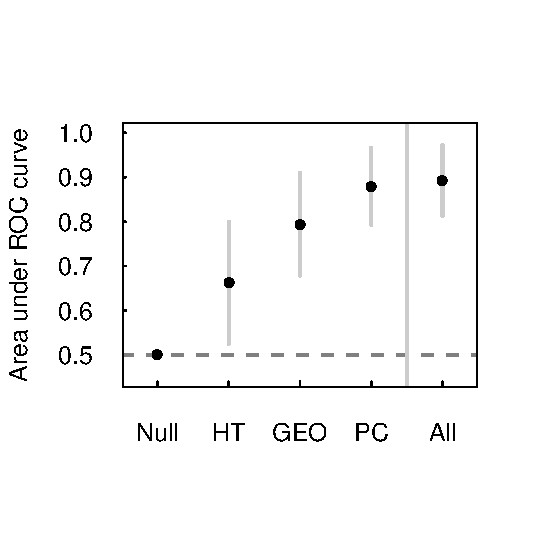
\includegraphics[width=\textwidth]{Figures/brtAccuracy.pdf}
  \caption{Accuracy (Area under Receiver operator characteristic (ROC) curves) for our predictive models incorporating host traits ('HT'),  our null model ('Null') that maintained interaction number (number of occurrence records), but assigned occurrences equiprobably among potential interactors.}
 \label{fig:brtAccuracy}
 \end{figure}

\newpage
 \begin{figure}[h!]
  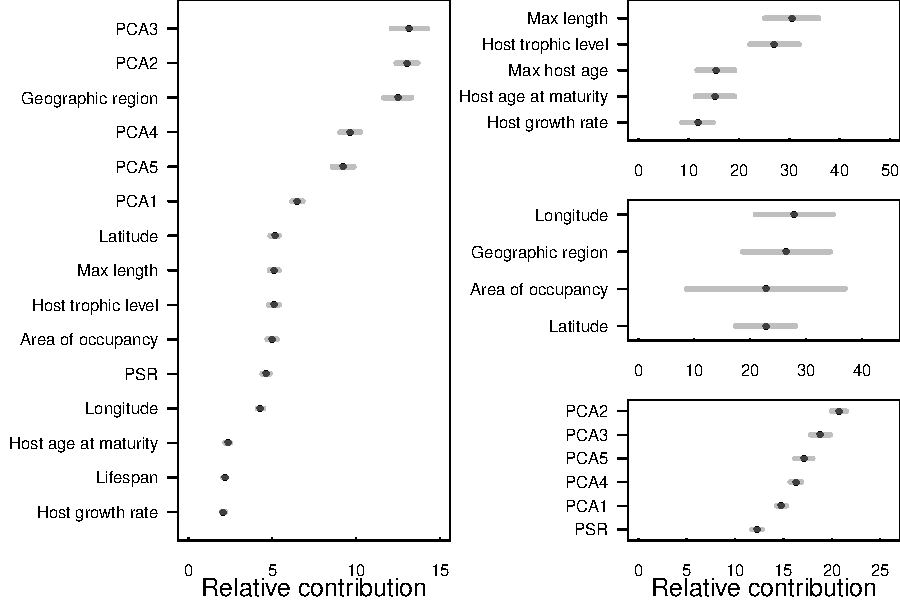
\includegraphics[width=\textwidth]{Figures/megaBRT.pdf}
  \caption{The average relative contribution values from the boosted regression tree models trained on all available data (left), host trait data (top right), geographic variables (middle right), and parasite community similarity (bottom right). Variables named ``PCA'' are principal components axes, and ``PSR'' refers to parasite species richness. Other variable definitions and units are available in Table 1. }
 \label{fig:megaBRT}
 \end{figure}

 \newpage
  %I like this plot because it's pretty, but I worry that any new information is just getting lost in the rainbow soup. Another idea would be to just color code classes of variables to highlight the importance of parasite community similarity. 
 \begin{figure}[h!]
  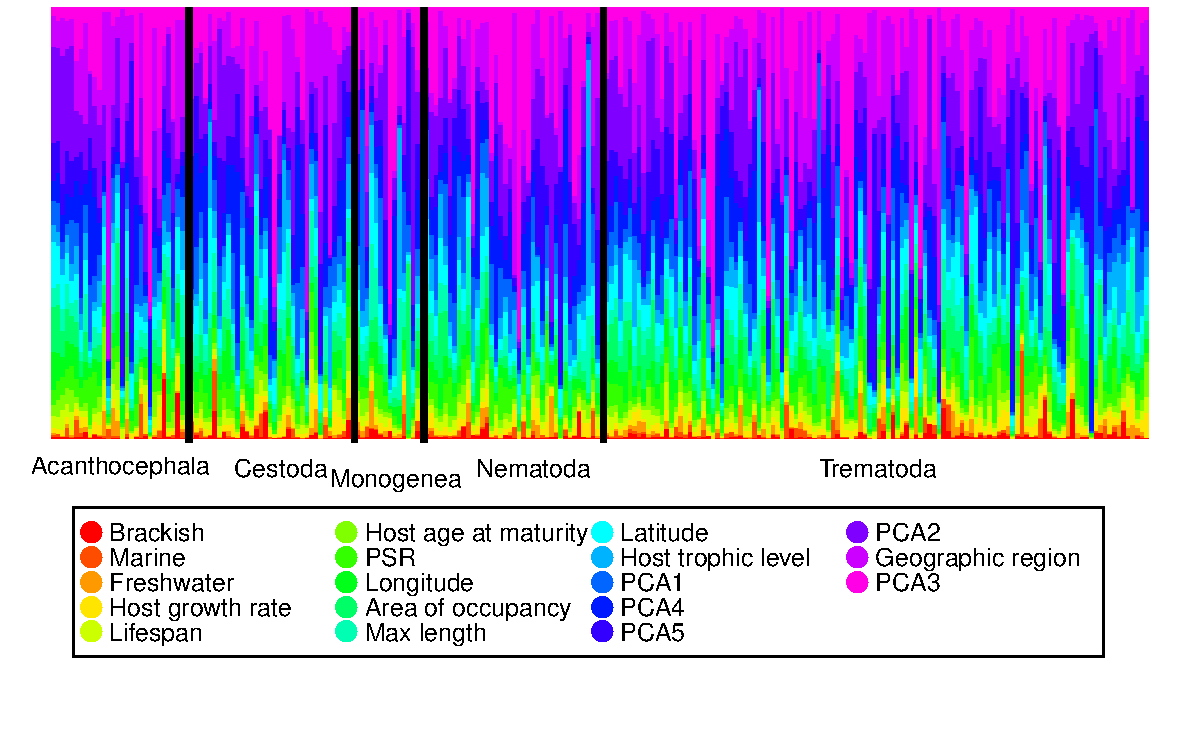
\includegraphics[width=\textwidth]{Figures/parTypeColor.pdf}
  \caption{Variation in variable importance as a function of parasite type. Each column represents a model trained on occurrence data for a single parasite species. Variables are sorted by their mean relative importance values across parasite species, but these values vary among parasite species.}
 \label{fig:parType}
 \end{figure}


 
 
 


\newpage
\section{Supplementary Material}

\begin{figure}[h]
  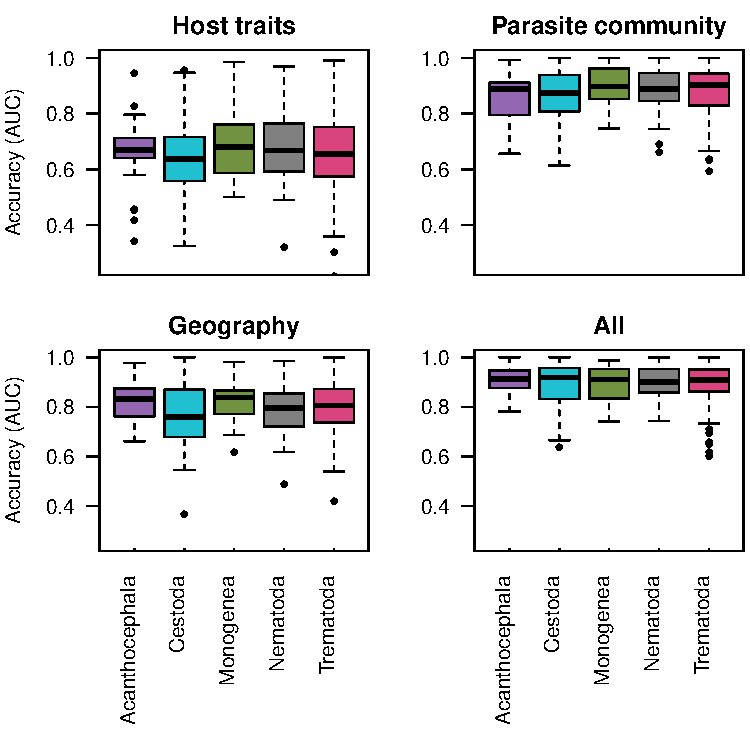
\includegraphics[width=\textwidth]{Figures/parAccuracy.pdf}
  \caption{Accuracy (Area under Receiver operator characteristic (ROC) curves) for boosted regression models trained using host traits (top left), parasite community similarity (top right), geographic variables (bottom left), and all available data (bottom right) as a function of parasite type ($x$-axis).   }
 \label{fig:parasite}
 \end{figure}







\end{document}
-